% -*- pdf: BrettTerespolskyMScDissertation.pdf -*-
%%%%%%%%%%%%%%%%%%%%%%%%%%%%%%%%%%%%%%%%%
% Thesis
% LaTeX Template
% Version 1.4 (30/6/13)
%
% This template has been downloaded from:
% http://www.latextemplates.com
%
% Original authors:
% Steven Gunn
% http://users.ecs.soton.ac.uk/srg/softwaretools/document/templates/
% and
% Sunil Patel
% http://www.sunilpatel.co.uk/thesis-template/
%
% License:
% CC BY-NC-SA 3.0 (http://creativecommons.org/licenses/by-nc-sa/3.0/)
%
% Note:
% Make sure to edit document variables in the Thesis.cls file
%
%%%%%%%%%%%%%%%%%%%%%%%%%%%%%%%%%%%%%%%%%

%----------------------------------------------------------------------------------------
%	PACKAGES AND OTHER DOCUMENT CONFIGURATIONS
%----------------------------------------------------------------------------------------

\documentclass[11pt, a4paper, oneside]{Thesis} % Paper size, default font size and one-sided paper
\usepackage{etex}

\graphicspath{{./Figures/}} % Specifies the directory where pictures are stored

\usepackage[square, numbers, comma, sort&compress]{natbib} % Use the natbib reference package - read up on this to edit the reference style; if you want text (e.g. Smith et al., 2012) for the in-text references (instead of numbers), remove 'numbers'
\usepackage{har2nat}
\makeatletter
\def\@mb@citenamelist{cite,citep,citet,citealp,citealt}
\makeatother
\usepackage{multibib}
\newcites{bib}{Bibliography}
\renewcommand{\bibname}{References}
\usepackage{tocbibind}
\usepackage[inline]{trackchanges}
% trackchanges package options:
% finalold  - Reject all edits. Refrain from using this.
% finalnew  - Accept all edits. Refrain from using this.
% The above two options should not be used, rather the trackchanges.py application must be used. Alternatively there is the acceptchanges.py for the terminal but check options carefully
% footnotes - Display edits as footnotes.
% margins   - Display edits as margin notes.
% inline    - Display edits inline.
\addeditor{KJN}
\addeditor{BRT}
% Usage of trackchanges below
% \add[editor]{added text}
% \remove[editor]{removed text}
% \change[editor]{removed text}{added text}
% \note[editor]{note text}
% \annote[editor]{text to annotate}{note text}
\makeatletter
\def\input@path{{./Primitives/}}
\makeatother
\usepackage{tikz}
\usepackage{pgfplots}
\usepackage{circuitikz}
\pgfplotsset{compat=1.10}
\usetikzlibrary{shapes.geometric, intersections,arrows}
\usepgfplotslibrary{external}
\usetikzlibrary{matrix}
\usepgfplotslibrary{groupplots}
\usepackage{pdfpages}
\tikzexternalize[prefix=TikzFigures/,shell escape=-enable-write18,optimize command away=\includepdf] %  activate!

\usepackage[toc, acronym, nonumberlist, nopostdot]{glossaries}
\newglossarystyle{mylong}{
\glossarystyle{long}
    \renewenvironment{theglossary}%
        {\begin{longtable}{p{0.35\linewidth}p{0.6\linewidth}}}%
        {\end{longtable}}%
    \renewcommand*{\glossaryentryfield}[5]{%
        \glsentryitem{##1}\glstarget{##1}{##2} & ##3\glspostdescription\space ##5\\[7.5pt]}%
}
\glossarystyle{mylong}
\renewcommand{\glsnamefont}[1]{\textbf{#1}}

\makeglossaries

\usepackage{subfigure}
\usepackage{breqn}

\usepackage{Extras}

\hypersetup{urlcolor=blue, colorlinks=false} % Colors hyperlinks in blue - change to black if annoying
\title{\ttitle} % Defines the thesis title - don't touch this

%----------------------------------------------------------------------------------------
%	Allow Russian alphabet from english letters. Just type \textcry{...}
%----------------------------------------------------------------------------------------
\usepackage[OT2,T1]{fontenc}
\newcommand\textcyr[1]{{\fontencoding{OT2}\fontfamily{wncyr}\selectfont #1}}
\def\Eoborotnoye{\char3}
\def\eoborotnoye{\char11}
\def\cprime{\char126}
\def\cdprime{\char127}

\newacronym[]{lps}{LPS}{Lightning Protection System}
\newacronym[]{lemp}{LEMP}{Lightning Electromagnetic Pulse}
\newacronym[]{lpl}{LPL}{Lightning Protection Level}

\newglossaryentry{heidler}
{
    name=Heidler function,
    description={A function used to generate lightning impulse currents. There are several parameters that can be changed to manipulate the rise and fall times of the waveshape. This function is stipulated in the IEC~62305-1 standard as the standardised lightning impulse current model used for Lightning Protection System design.}
}
\newglossaryentry{approx}
{
    name=Heidler function approximation,
    description={The function developed in this dissertation that approximates the Hediler function with an analytical integral.}
}
\newglossaryentry{waveshape}
{
    name=Waveshape,
    description={The shape of a graph in the time domain.}
}
\newglossaryentry{iec}
{
    name=IEC~62305,
    description={The lightning protection standard.}
}
\newglossaryentry{iec1}
{
    name=IEC~62305-1,
    description={Part one of the IEC~62305. This details all the parameters of lightning currents and the nomenclature used in lightning current models. This standard also details the first and subsequent short strokes and how they can be simulated using the Heidler function.}
}
\newglossaryentry{lsm}
{
    name=Lightning stroke model,
    description={A mathematical model used to represent a lightning current waveshape. Examples of these are the Heidler function, the double exponential function and the approximation to the Heidler function that is represented in this dissertation.}
}
\newglossaryentry{short}
{
    name=Short stroke,
    description={A component of a lightning stroke that is impulsive in nature unlike the long stroke which is a comparatively long sustained current.}
}
\newglossaryentry{fs}
{
    name=First short stroke,
    description={A short stroke that is defined by the IEC~62305-1 as having a rise time of 10~\usec and a decay time of 350~\usec.}
}
\newglossaryentry{ss}
{
    name=Subsequent short stroke,
    description={A short stroke that is defined by the IEC~62305-1 as having a rise time of 0.25~\usec and a decay time of 100~\usec.}
}
\newglossaryentry{rtc}
{
    name=Rise time constant,
    description={A constant that is used to change the rise time of the lightning current waveshape.}
}
\newglossaryentry{dtc}
{
    name=Decay time constant,
    description={A constant that is used to change the decay time (the time to 50\% of peak current) of the lightning current waveshape.}
}
\newglossaryentry{rtf}
{
    name=Rise time function,
    description={The function that dictates what the shape of the rise of the waveshape is.}
}
\newglossaryentry{dtf}
{
    name=Decay time function,
    description={The function that dictates what the shape of the decay of the waveshape is.}
}
\newglossaryentry{steep}
{
    name=Waveshape steepness,
    description={A higher steepness in a waveshape results in a larger maximum instantaneous change in current.}
}

\glsaddall

\begin{document}

\frontmatter % Use roman page numbering style (i, ii, iii, iv...) for the pre-content pages

\setstretch{1.3} % Line spacing of 1.3

% Define the page headers using the FancyHdr package and set up for one-sided printing
\fancyhead{} % Clears all page headers and footers
\rhead{\thepage} % Sets the right side header to show the page number
\lhead{} % Clears the left side page header

\pagestyle{fancy} % Finally, use the "fancy" page style to implement the FancyHdr headers

\newcommand{\HRule}{\rule{\linewidth}{0.5mm}} % New command to make the lines in the title page

% PDF meta-data
\hypersetup{pdftitle={\ttitle}}
\hypersetup{pdfsubject=\subjectname}
\hypersetup{pdfauthor=\authornames}
\hypersetup{pdfkeywords=\keywordnames}

%----------------------------------------------------------------------------------------
%	TITLE PAGE
%----------------------------------------------------------------------------------------

\maketitle

%----------------------------------------------------------------------------------------
%	DECLARATION PAGE
%	Your institution may give you a different text to place here
%----------------------------------------------------------------------------------------

\Declaration{

\addtocontents{toc}{\vspace{1em}} % Add a gap in the Contents, for aesthetics

I, \authornames, declare that this dissertation titled, `\ttitle'  is my own unaided work. It is being submitted to the Degree of Master of Science to the University of the Witwatersrand, Johannesburg. It has not been submitted before for any degree or examination to any other University.

\vfill

Signed:\\
\rule[1em]{25em}{0.5pt} % This prints a line for the signature

Date:\\
\rule[1em]{25em}{0.5pt} % This prints a line to write the date
}

\clearpage % Start a new page

%----------------------------------------------------------------------------------------
%	QUOTATION PAGE
%----------------------------------------------------------------------------------------

\pagestyle{empty} % No headers or footers for the following pages

\null\vfill % Add some space to move the quote down the page a bit

\textit{``Give me six hours to chop down a tree and I will spend the first four sharpening the axe."}

\begin{flushright}
Abraham Lincoln
\end{flushright}

\vfill\vfill\vfill\vfill\vfill\vfill\null % Add some space at the bottom to position the quote just right

\clearpage % Start a new page

%----------------------------------------------------------------------------------------
%	ABSTRACT PAGE
%----------------------------------------------------------------------------------------

\addtotoc{Abstract} % Add the "Abstract" page entry to the Contents

\abstract{\addtocontents{toc}{\vspace{1em}} % Add a gap in the Contents, for aesthetics

The work presented contributes to research in lightning protection simulations and focuses on approximating the Heidler function with an analytical integral and hence a frequency domain representation. The integral of lightning current models is required in the analysis of lightning events including the induced effects and frequency analyses of lightning strikes. Previous work in this area has produced very specific forms of the Heidler function that are used to represent lightning current waveshapes. This work however focuses on a generic solution with parameters that can be modified to produce any lightning current waveshape that is required. In the research presented, such an approximation is obtained. This function has an analytical solution to the integral and hence can be completely represented in the frequency domain. This allows for a true representation of Maxwell's equations for \gls{em} fields and for an analytical frequency domain analysis. It has parameters that can be changed to obtain different waveshapes (10/350, 0.25/100, etc.). The characteristics of the approximation are compared with those of the Heidler function to ascertain whether or not the function is applicable for use with the lightning protection standard (IEC~62305-1). It is shown that the approximation does represent the same characteristics as those of the Heidler function and hence can be used in IEC~62305-1 standardised applications. This represents a valuable contribution to engineers working in the field of lightning protection, specifically simulation models.

\clearpage % Start a new page

%----------------------------------------------------------------------------------------
%	ACKNOWLEDGEMENTS
%----------------------------------------------------------------------------------------

\setstretch{1.3} % Reset the line-spacing to 1.3 for body text (if it has changed)

\acknowledgements{\addtocontents{toc}{\vspace{1em}} % Add a gap in the Contents, for aesthetics

The acknowledgements and the people to thank go here, don't forget to include your project advisor\ldots
}
\clearpage % Start a new page

%----------------------------------------------------------------------------------------
%	LIST OF CONTENTS/FIGURES/TABLES PAGES
%----------------------------------------------------------------------------------------

\pagestyle{fancy} % The page style headers have been "empty" all this time, now use the "fancy" headers as defined before to bring them back

\lhead{\emph{Contents}} % Set the left side page header to "Contents"
\tableofcontents % Write out the Table of Contents

\clearpage
\lhead{\emph{List of Figures}} % Set the left side page header to "List of Figures"
\listoffigures % Write out the List of Figures

\clearpage
\lhead{\emph{List of Tables}} % Set the left side page header to "List of Tables"
\listoftables % Write out the List of Tables

%----------------------------------------------------------------------------------------
%	ABBREVIATIONS
%----------------------------------------------------------------------------------------

\clearpage % Start a new page

\setstretch{1.5} % Set the line spacing to 1.5, this makes the following tables easier to read

% \lhead{\emph{Abbreviations}} % Set the left side page header to "Abbreviations"
% \printglossary[type=\acronymtype, title=Abbreviations]

%----------------------------------------------------------------------------------------
%	PHYSICAL CONSTANTS/OTHER DEFINITIONS
%----------------------------------------------------------------------------------------

% \clearpage % Start a new page

% \lhead{\emph{Physical Constants}} % Set the left side page header to "Physical Constants"

% \listofconstants{lrcl} % Include a list of Physical Constants (a four column table)
% {
% Speed of Light & $c$ & $=$ & $2.997\ 924\ 58\times10^{8}\ \mbox{ms}^{-\mbox{s}}$ (exact)\\
% % Constant Name & Symbol & = & Constant Value (with units) \\
% }

%----------------------------------------------------------------------------------------
%	SYMBOLS
%----------------------------------------------------------------------------------------

\clearpage % Start a new page

\lhead{\emph{Symbols}} % Set the left side page header to "Symbols"

\listofnomenclature{lll} % Include a list of Symbols (a three column table)
{
% \textbf{Symbol} & \textbf{Description} & \textbf{Units} \\
% & & \\ % Gap
\multicolumn{3}{l}{\textbf{Electromagnetic Equations of a Lightning Stroke}} \\
$E_z \left( D, t \right)$ & Electric field & V/m \\
$B_{\phi} \left( D,t \right)$ & Magnetic field & T \\

& & \\ % Gap
\multicolumn{3}{l}{\textbf{Lightning Current Return Stroke Modelling}} \\
$i \left( z',t \right)$ & Lightning current return stroke model & A \\
$i \left( 0,t \right)$ & Lightning channel base current & A \\

& & \\ % Gap
\multicolumn{3}{l}{\textbf{Double Exponential Function}} \\
$i_e \left( t \right)$ & Double exponential lightning stroke current model & A \\
$I_0$ & Peak current & A \\
$A$ & Double exponential peak current correction &  \\
$\alpha$ & Double exponential decay time constant & 1/s \\
$\beta$ & Double exponential rise time constant & 1/s \\

& & \\ % Gap
\multicolumn{3}{l}{\textbf{Heidler Function}} \\
$i_h \left( t \right)$ & Heidler function lightning stroke current model & A \\
$\eta$ & Peak current correction &  \\
$\tau_1$ & Heidler rise time constant & s \\
$\tau_2$ & Decay time constant & s \\
$n_h$ & Heidler steepness factor & \\
$i'_h \left( t \right)$ & First time derivative of $i_h \left( t \right)$ & A/s \\
$x_h \left( t \right)$ & Heidler function rise time function &  \\
$y \left( t \right)$ & Decay function & \\

& & \\ % Gap
\multicolumn{3}{l}{\textbf{Heidler Function Approximation}} \\
$X_a \left( s \right)$ & Rise time function of the approximation (Laplace domain) &  \\
$x_a \left( t \right)$ & Rise time function of the approximation (time domain) &  \\
$i_a \left( t \right)$ & Approximated lightning stroke current model & A \\
$\omega_0$ & Rise time constant of the approximation & rad/s \\
$n_a$ & Steepness factor of the approximation & \\
$i'_a \left( t \right)$ & First time derivative of $i_a \left( t \right)$ & A/s \\
$I_a \left( j\omega \right)$ & Fourier transform (angular frequency) of $i_a \left( t \right)$ &  \\
$I_a \left( jf \right)$ & Fourier transform (linear frequency) of $i_a \left( t \right)$ & A/Hz \\

& & \\ % Gap
\multicolumn{3}{l}{\textbf{Error Evaluation}} \\
$e \left( s \right)$ & Error function & A \\
$e' \left( t \right)$ & First time derivative of $e \left( t \right)$ & A/s \\

% Symbol & Name & Unit \\

% & & \\ % Gap to separate the Roman symbols from the Greek

% $\omega$ & angular frequency & rads$^{-1}$ \\
% Symbol & Name & Unit \\
}

%----------------------------------------------------------------------------------------
%    Nomenclature
%----------------------------------------------------------------------------------------

\clearpage % Start a new page

\lhead{\emph{Nomenclature}} % Set the left side page header to "Abbreviations"
\printglossary[title=Nomenclature]


%----------------------------------------------------------------------------------------
%	DEDICATION
%----------------------------------------------------------------------------------------

\clearpage

\setstretch{1.3} % Return the line spacing back to 1.3

\pagestyle{empty} % Page style needs to be empty for this page

\dedicatory{For/Dedicated to/To my\ldots \textcyr{Privet SHurochka\\
a b v g d e \"e zh z i\\ {\u i} k l m n o p r s t\\ u f kh c ts
shch ch sh y yu\\ ya
\Eoborotnoye~
\eoborotnoye~
\cprime~
\cdprime~
}} % Dedication text

\addtocontents{toc}{\vspace{2em}} % Add a gap in the Contents, for aesthetics

%----------------------------------------------------------------------------------------
%	THESIS CONTENT - CHAPTERS
%----------------------------------------------------------------------------------------

\mainmatter % Begin numeric (1,2,3...) page numbering

\pagestyle{fancy} % Return the page headers back to the "fancy" style

% Include the chapters of the thesis as separate files from the Chapters folder
% Uncomment the lines as you write the chapters

% -*- root: ../main.tex -*-
% Chapter Template

\chapter{Introduction} % Main chapter title

\label{ChapterIntro} % Change X to a consecutive number; for referencing this chapter elsewhere, use \ref{ChapterX}

\lhead{\chaptername~\thechapter. \emph{Introduction}} % Change X to a consecutive number; this is for the header on each page - perhaps a shortened title

Mathematical lightning current models are used in many areas of research ranging from the design of lightning protection systems to the understanding of electric and magnetic fields associated with lightning discharges \cite{IEC623051, ZhangFeizhouandLiuShanghe2002}.
Lightning current models are typically used as design tools and for further research into the understanding of the effects of a lightning strike.
They have become an integral part of lightning research and Lightning Protection System (LPS) design.
This research provides an approximation to the Heidler function that can be integrated. This allows for an accurate frequency domain representation of the function. Furthermore, the electromagnetic fields can be calculated using Maxwell's equations analytically.

An equation is designed to approximate the Heidler function. The function is as ``customisable'' as the Heidler function (i.e. any lightning current waveshape can be obtained with varying characteristics).
An investigation is carried out to determine the accuracy of the approximation. This is done by using computer simulations of the approximation and the results are compared to the Heidler function and the IEC~62305 lightning protection standard to determine the viability of this approximation in the design of LPSs.

\chapref{ChapterApproach} details the \textbf{\textit{approach taken}} in designing and evaluating the approximation to the Heidler function. The assumptions and constraints made in this study are outlined. The significance of this study in the field of lightning research is discussed with reference to the problem statements.

\chapref{ChapterBackground} discusses the relevant \textbf{\textit{background}} information with respect to this research. This includes information about the Heidler function and the Lightning Electromagnetic Pulse (LEMP) equations. A review of the existing work in the field of approximating lightning currents is also identified.

\chapref{ChapterApprox} provides the actual \textbf{\textit{approximation to the Heidler function}}. All the components of the equation are discussed as well as the parameters used to create the various waveshapes. A comparison of the parameters used in the approximation and the Heidler function are given. Some results of the approximation are simulated and detailed in this chapter.

\chapref{ChapterResults} investigates the accuracy of the approximation by simulating \textbf{\textit{results}} and comparing them to the expected values obtained from the Heidler function. Furthermore the characteristics such as maximum instantaneous change in current, charge, etc. are compared to those outlined in the IEC~62305 standard.

\chapref{ChapterDiscussion} summarises the results obtained from the simulations. A \textbf{\textit{discussion}} of the viability of this approximation as a suitable replacement to the Heidler function is provided. \textbf{\textit{Future work}} in the field of approximating lightning current models is detailed with the goal of optimising the approximation detailed in this study.

\chapref{ChapterConclusion} provides a \textbf{\textit{conclusion}} to the work and discusses the viability of this function in various fields of lightning research.

% -*- root: ../main.tex -*-
% Chapter Template

\chapter{Approach Taken} % Main chapter title

\label{ChapterApproach} % Change X to a consecutive number; for referencing this chapter elsewhere, use \ref{ChapterX}

\lhead{\chaptername~\thechapter. \emph{Approach Taken}} % Change X to a consecutive number; this is for the header on each page - perhaps a shortened title

%----------------------------------------------------------------------------------------
%	SECTION 1
%----------------------------------------------------------------------------------------

\section{Main Section 1}

Lorem ipsum dolor sit amet, consectetur adipiscing elit. Aliquam ultricies lacinia euismod. Nam tempus risus in dolor rhoncus in interdum enim tincidunt. Donec vel nunc neque. In condimentum ullamcorper quam non consequat. Fusce sagittis tempor feugiat. Fusce magna erat, molestie eu convallis ut, tempus sed arcu. Quisque molestie, ante a tincidunt ullamcorper, sapien enim dignissim lacus, in semper nibh erat lobortis purus. Integer dapibus ligula ac risus convallis pellentesque.

%-----------------------------------
%	SUBSECTION 1
%-----------------------------------
\subsection{Subsection 1}

Nunc posuere quam at lectus tristique eu ultrices augue venenatis. Vestibulum ante ipsum primis in faucibus orci luctus et ultrices posuere cubilia Curae; Aliquam erat volutpat. Vivamus sodales tortor eget quam adipiscing in vulputate ante ullamcorper. Sed eros ante, lacinia et sollicitudin et, aliquam sit amet augue. In hac habitasse platea dictumst.

%-----------------------------------
%	SUBSECTION 2
%-----------------------------------

\subsection{Subsection 2}
Morbi rutrum odio eget arcu adipiscing sodales. Aenean et purus a est pulvinar pellentesque. Cras in elit neque, quis varius elit. Phasellus fringilla, nibh eu tempus venenatis, dolor elit posuere quam, quis adipiscing urna leo nec orci. Sed nec nulla auctor odio aliquet consequat. Ut nec nulla in ante ullamcorper aliquam at sed dolor. Phasellus fermentum magna in augue gravida cursus. Cras sed pretium lorem. Pellentesque eget ornare odio. Proin accumsan, massa viverra cursus pharetra, ipsum nisi lobortis velit, a malesuada dolor lorem eu neque.

%----------------------------------------------------------------------------------------
%	SECTION 2
%----------------------------------------------------------------------------------------

\section{Main Section 2}

Sed ullamcorper quam eu nisl interdum at interdum enim egestas. Aliquam placerat justo sed lectus lobortis ut porta nisl porttitor. Vestibulum mi dolor, lacinia molestie gravida at, tempus vitae ligula. Donec eget quam sapien, in viverra eros. Donec pellentesque justo a massa fringilla non vestibulum metus vestibulum. Vestibulum in orci quis felis tempor lacinia. Vivamus ornare ultrices facilisis. Ut hendrerit volutpat vulputate. Morbi condimentum venenatis augue, id porta ipsum vulputate in. Curabitur luctus tempus justo. Vestibulum risus lectus, adipiscing nec condimentum quis, condimentum nec nisl. Aliquam dictum sagittis velit sed iaculis. Morbi tristique augue sit amet nulla pulvinar id facilisis ligula mollis. Nam elit libero, tincidunt ut aliquam at, molestie in quam. Aenean rhoncus vehicula hendrerit.
% -*- root: ../main.tex -*-
% Chapter Template

\chapter{Background} % Main chapter title

\label{ChapterBackground} % Change X to a consecutive number; for referencing this chapter elsewhere, use \ref{ChapterX}

\lhead{\chaptername~\thechapter. \emph{Background}} % Change X to a consecutive number; this is for the header on each page - perhaps a shortened title
\begin{quote}
\note[BRT]{Chapter abstract goes here!}
\end{quote}

%----------------------------------------------------------------------------------------
%    Overview
%----------------------------------------------------------------------------------------

\section{Overview}
\label{sec:background_overview}


%----------------------------------------------------------------------------------------
%    Application for Lightning Current Models
%----------------------------------------------------------------------------------------

\section{Application for Lightning Current Models}
\label{sec:background_applications}
There are several instances when there is a requirement to use a lightning current model. When designing \glspl{lps}, there is a need for lightning current model. Two of the more specific cases where lightning current models are used are detailed below. These include current path analyses using return stroke modelling and the need for the frequency components of lightning.
%-----------------------------------
%    Current Path Analyses
%-----------------------------------
\subsection{Current Path Analyses}
\label{sub:background_lemp}
Return stroke models are characterised into four primary classes, namely gas dynamics model, electromagnetic model, distributed circuit model and the engineering model \cite{Paolone2009,Rakov2003,Rakov2009}. However the engineering model is the primary model when looking at induced effects on power lines.

\begin{figure}[htbp]
    \centering
    \subfigure[]{
        \tikzsetnextfilename{PhysicalModel}
        %!tikz editor 1.0
%!tikz source begin
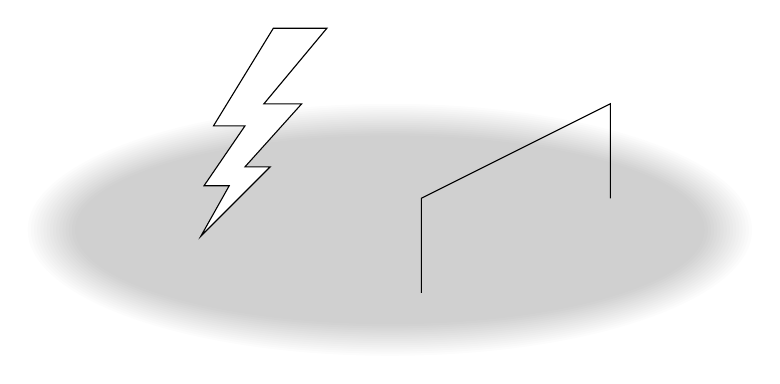
\begin{tikzpicture}[scale=0.8, transform shape]
%\fill [black, fill opacity = 0.075] (2,0.8) ellipse [x radius = 5, y radius = 1.5];

\foreach \i in {0,2,...,30}
        \fill [black, fill opacity = 1/100] (2,0.8)
          ellipse [x radius = 5+\i/40, y radius = 1.5+\i/60];

\fill [draw,fill=white] (1,4) to ++ (-1,-1.2) to ++ (0.6,0) to ++ (-0.9,-1) to ++ (0.4,0) to ++ (-1.1, -1.1) node (bot) {} to ++ (0.45,0.8) to ++ (-0.4,0) to ++ (0.65,0.95) to ++ (-0.5,0) to ++ (0.95,1.55) -- cycle;

\draw (bot) ++ (3.5,-0.9) to ++ (0,1.5) to ++(3,1.5) to ++ (0,-1.5);
\end{tikzpicture}
%!tikz source end

        \label{fig:physical_model}
    }
    \subfigure[]{
        \tikzsetnextfilename{TransmissionLineModel}
        %!tikz editor 1.0
%!tikz source begin
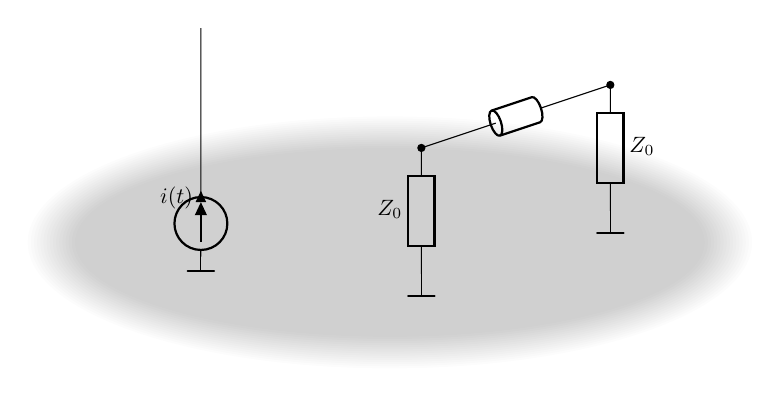
\begin{tikzpicture}[american currents, scale=0.8, transform shape]
\foreach \i in {0,2,...,30}
        \fill [black, fill opacity = 1/100] (2,0.8)
          ellipse [x radius = 5+\i/40, y radius = 1.5+\i/60];

\fill [fill=none] (1,4) to ++ (-1,-1.2) to ++ (0.6,0) to ++ (-0.9,-1) to ++ (0.4,0) to ++ (-1.1, -1.1) node (bot) {} to ++ (0.45,0.8) to ++ (-0.4,0) to ++ (0.65,0.95) to ++ (-0.5,0) to ++ (0.95,1.55) -- cycle;

\draw (bot) node[rground] {} to [I=$i(t)$] ++ (0,0.8) to ++(0,2.7);

\draw (bot) ++ (3.5,-0.4) node[rground]{} to[generic=$Z_0$] +(0,2);
\draw (bot) ++ (6.5,2.6) to[transmission line, *-*]++(-3,-1);
\draw (bot) ++ (6.5,2.6) to[generic=$Z_0$] ++ (0,-2) node[rground]{};

\end{tikzpicture}
%!tikz source end

        \label{fig:tr_line_model}
    }
    \caption[]{\subref{fig:physical_model} Physical and \subref{fig:tr_line_model} Transmission Line models of a lightning strike close to a transmission line that induces over-voltages on the line.}
    \label{fig:induced_voltage_models}
\end{figure}
\figref{fig:induced_voltage_models} shows the \subref{fig:physical_model} physical and \subref{fig:tr_line_model} return stroke models for a lightning strike in close proximity to a transmission line. From these figures it can be seen that when modelling a lightning strike occurring in close proximity to a transmission line, the lightning channel is modelled as a monopole with a perfectly conductive ground and a vertical current path \cite{Paolone2009,Baba2007,McAfee2015}.

Information about the \gls{em} fields are required when calculating the induced effects of the lightning strike on the transmission line. By integrating the different components of the \gls{em} fields as outline by \citeauthor{Agrawal1980}, the induced currents can be calculated \cite{Agrawal1980}. In order to obtain the \gls{em} fields however, the \gls{lemp} equations need to be determined. The equations for the electric and magnetic fields can be seen in \eqnrefs{eqn:e_field}{eqn:b_field} respectively. These are defined by \citeauthor{Uman1975} as the \gls{lemp} equations \cite{Uman1975}.
\begin{dmath}
    E_z \left( D,t \right)=\frac{1}{2\pi\epsilon_0}\left[\int_{0}^{H}\frac{2 - 3\sin^{2}{\theta}}{R^3} \times \int_{0}^{t} i \left( z, \tau - \frac{R}{c} \right) \, d\tau dz \\ + \int_{0}^{H} \frac{2 - 3\sin^{2}{\theta}}{c R^2} i \left( z, t - \frac{R}{c} \right) \, dz - \int_{0}^{H} \frac{\sin^{2}{\theta}}{c^2 R} \frac{\partial i\left ( z, t - \frac{R}{c} \right )}{\partial t} \, dz \right ]
    \label{eqn:e_field}
\end{dmath}
\begin{dmath}
    B_{\phi} \left( D,t \right) = \frac{\mu_0}{2\pi} \int_{0}^{H} \frac{\sin{\theta}}{R^2} i \left ( z, t - \frac{r}{c} \right ) \, dz + \frac{\mu_0}{2\pi} \int_{0}^{H} \frac{\sin{\theta}}{cR} \frac{\partial i \left ( z, t - \frac{R}{c} \right )}{\partial t} \, dz
    \label{eqn:b_field}
\end{dmath}
The full extent of what these equations mean is beyond the scope of this study. However, what is clear is that these equations utilise the return stroke model, $i \left( z, t \right)$. This expression for the lightning current along a path can be defined by different models as in \cite{Paolone2009,ZhangFeizhouandLiuShanghe2002,Nucci2003}. All the models hold the form shown in \eqnref{eqn:rsm} where $u(t)$ is the Heaviside function, $P(z')$ is the height-dependent current attenuation factor and $i(0,t)$ is the lightning channel base current which as the name suggests is the current as measured from the base of the object that is struck \cite{Paolone2009,ZhangFeizhouandLiuShanghe2002,Javor2011}.
\begin{equation}
    i(z',t)=u\left( t - \frac{z'}{v}\right) P \left( z' \right) i \left( 0,t - \frac{z'}{v} \right)
    \label{eqn:rsm}
\end{equation}
In short, there are two steps of integration required to calculate induced currents on transmission lines \cite{Nucci2010,Nucci2003,Paolone2009}.
\begin{enumerate}
    \item Integrate some model of the lightning channel base current to obtain the \gls{em} fields.
    \item Integrate the electric fields using the equations defined by \citeauthor{Agrawal1980} to obtain the induced currents.
\end{enumerate}

Therefore, by choosing an appropriate lightning channel base current, the induced effects on nearby transmission lines can be calculated. Clearly from the equations above, at least the second integral of this channel base current is required. Using an accurate lightning channel base current leads to very complex models that require long computer simulations because of numerical integration \cite{Paolone2009}. \secref{sec:background_current_waveshape_models} details two of the more common equations used as lightning channel base current models.

%-----------------------------------
%    Frequency Components of Lightning Currents
%-----------------------------------
\subsection{Frequency Components of Lightning Currents}
\label{sub:background_frequency_components_of_lightning_currents}
Obtaining frequency components of a lightning strike are important for studies such as that done by \citeauthor{Lee2014}, where they are studying the effects of the lightning frequency components on human injury caused by a lightning strike \cite{Lee2014}. In this study, \citeauthor{Lee2014} utilise the double exponential function to obtain the frequency components of a lightning strike. The frequency components in the double exponential are found to be an order of magnitude different to those recommended by the standards \cite{1422588}.

The reason for such a study is that the sharp rise in the lightning current creates a broadband current. Without using the Heidler function for such applications, it is difficult to standardise testing across the different fields of interest.

%----------------------------------------------------------------------------------------
%    IEC~62305 - Lightning Protection Standard
%----------------------------------------------------------------------------------------

\section{IEC~62305-1 - Lightning Protection Standard}
\label{sec:background_iec62305}
The IEC~62305-1 is part one of the lightning protection standard. It focuses on the general principles of lightning protection. Parts two to four focus on more specific areas of lightning protection. This standard details all the relevant components of a lightning flash as well as all the terminology and standard values to utilise when designing systems such as \glspl{lps}.

\figref{fig:IECWave} shows an adaptation of Figure A.1 from the standard. This figure shows how the different stroke currents, such as the 0.25/100 and 10/350 are composed. $T_1$ is the rise time (number before the `/') and $T_2$ is the fall time (number after the `/').
\inputtikzfig{IECWave}{IECWave}{Definitions of short stroke parameter adapted from \cite{IEC623051}}

Figures A.3 and A.4 in the standard show typical waveshapes expected from both downward and upward lightning flashes respectively. The three components identified in these images are the first short stroke, the subsequent short stroke and the long stroke. The first and subsequent short strokes are seen to be high current impulses with a sharp rise and a slower decay. The long stroke on the other hand is a lower current that is maintained for a comparatively long time.

Table A.1 in the standard shows the values that should be used in system designs. The values given here are the maximum change in current, the charge, the peak current, etc. With these values, systems can be designed to different \glspl{lpl}. The values given in this table are based on the original studies done by \citeauthor{Anderson1980} and \citeauthor{Berger1975} on lightning currents \cite{Anderson1980,Berger1975}. The standard typically makes use of the upper end values to protect against more cases.

In order to simulate lightning currents in \glspl{lps} design, the standard identifies a function that creates a waveshape with the characteristics outlined in Table A.1 of the standard. This function is the Heidler function with a specific configuration ($n = 10$) (see \secref{sub:background_heidler}). This function can be used to create any lightning current waveshape. The two of interest in the standard are the 10/350 (first short stroke) and the 0.25/100 (subsequent short stroke). These two waveshapes are simulated using the the parameters specified in Table B.1 for the different \glspl{lpl} and stroke types \cite{IEC623051}.

%----------------------------------------------------------------------------------------
%    Current Waveshape Models
%----------------------------------------------------------------------------------------

\section{Current Waveshape Models}
\label{sec:background_current_waveshape_models}
The IEC lightning protection standard details the Heidler function with a specific configuration as the standardised waveshape for lightning current simulations. There are however other lightning current models. The two most popular of these models are the Heidler and the double exponential. There are also applications that use some sort of combination of the two \cite{Javor2011,Nucci2003,Pavanello2007}. This section gives some background into these equations and their properties.

%-----------------------------------
%    The Double Exponential Model
%-----------------------------------
\subsection{The Double Exponential Model}
\label{sub:background_double_exponential}
The double exponential function is defined in \eqnref{eqn:dexp}.
\begin{equation}
    i_e \left( t \right) = \frac{I_o}{A}\left( e^{-\alpha t} - e^{-\beta t} \right)
    \label{eqn:dexp}
\end{equation}
Where: \\
\begin{tabular}{cll}
    $I_0$ & = & Peak current [A] \\
    $A$ & = & Peak current correction \\
    $\alpha$ & = & Decay time constant \\
    $\beta$ & = & Rise time constant
\end{tabular}\\
The double exponential model is often used in place of the Heidler function because it can be integrated. However the waveshape produced by the double exponential equation is not physically realistic. The maximum current steepness occurs at time $t=0$ \cite{ZhangFeizhouandLiuShanghe2002,Lovric2013,Heidler2002,Delfino2012}. Moreover, this function does not allow for waveshapes that comply with Table A.1 in the IEC~62305-1 standard. For instance, a subsequent short stroke for \gls{lpl} I would have a maximum current steepness of about 545 kA/\usec \cite{Heidler2008}. Another disadvantage to using this equation is that it is not easily adjustable, the parameters are not easily obtained \cite{Javor2011}.

%-----------------------------------
%    The Heidler Function
%-----------------------------------
\subsection{The Heidler Function}
\label{sub:background_heidler}
To avoid the disadvantages of the double exponential equation, the Heidler function is used. This can be seen in \eqnref{eqn:HF}.
\begin{equation}
i_h \left( t \right) = \frac{I_0}{\eta} \frac{{\left (\frac{t}{\tau_1} \right )}^{n_h}}{1 + {\left (\frac{t}{\tau_1} \right )}^{n_h}} e^{-\frac{t}{\tau_2}}
\label{eqn:HF}
\end{equation}

Where: \\
\begin{tabular}{cll}
    $I_0$ & = & Peak current [A] \\
    $\eta$ & = & Peak current correction \\
    $\tau_1$ & = & Rise time constant [\usec] \\
    $\tau_2$ & = & Decay time constant [\usec] \\
    $n_h$ & = & Steepness factor
\end{tabular}\\
This equation more realistically approximates a lightning return stroke \cite{ZhangFeizhouandLiuShanghe2002,Lovric2013,Delfino2012}. Furthermore, the peak current correction can be calculated using \eqnref{eqn:eta} \cite{Delfino2012,Javor2011,Heidler1999}.
\begin{equation}
    \eta =e^{-\frac{\tau _1}{\tau _2} \left(\frac{n_h \tau _2}{\tau _1}\right)^{\frac{1}{n_h}}}
    \label{eqn:eta}
\end{equation}
\eqnref{eqn:dHF} show the first derivative of the Heidler function.
\begin{equation}
    i'_h \left( t \right) = \frac{I_0}{\eta} \left( \frac{n_h t^{n_h - 1} \tau_1^{n_h}}{\left(\tau_1^{n_h} + t^{n_h} \right)^2} - \frac{t^{n_h}}{\tau_2 \left(\tau_1^{n_h} + t^{n_h} \right)} \right) e^{-\frac{t}{\tau_2}}
    \label{eqn:dHF}
\end{equation}

The IEC~62305-1 standard makes use of a specialised form of the Heidler function where $n_h = 10$. Using this form of the equation, there are values for the other parameters in the standard that can be used to simulate both first and subsequent short strokes \cite{IEC623051,Heidler2008}.

The disadvantage of the Heidler function is that there is no analytical integral and hence no analytical expression for the Heidler function in frequency domain \cite{ZhangFeizhouandLiuShanghe2002,Lovric2013}. This creates problems when trying to carry out analyses such as those mentioned in \secref{sec:background_applications} above.

%----------------------------------------------------------------------------------------
%    Heidler Function Approximations
%----------------------------------------------------------------------------------------

\section{Heidler Function Approximations}
\label{sec:background_approximations}
As there are is no analytical integral to the Heidler function, there are many researchers working towards an approximation that can be used in its place for applications such as those mentioned in \secref{sec:background_applications}. This section discusses a few of these approximations with the disadvantages associated with each one.

\citeauthor{ZhangFeizhouandLiuShanghe2002} developed a function that they call the \textit{Pulse function}. According to their study, this function produces a maximum error of 0.5\% with the waveshapes they used. However, this function is a modified form of the double exponential function. It requires very complex methods to determine the parameters used in the equation \cite{ZhangFeizhouandLiuShanghe2002}.

\citeauthor{Heidler2002} in \cite{Heidler2002}, approximates the Heidler function utilised in the IEC~62305-1 standard. This approximation has an analytical integral but the equation is specific to the subsequent short stroke. Moreover, there is no general form of this approximation and so this equation cannot be easily manipulated. That study also details several other approximations to the Heidler function but all with other applications. They all have the disadvantage that they cannot be integrated analytically.

\citeauthor{Delfino2012} conduct a study in which they develop a Prony series approximation to the Heidler function \cite{Delfino2012}. The mathematics required for this approximation is very complex. Each scenario is different as there is no truly generalised form. Furthermore the number of terms used affects the error associated with the approximation. This would be difficult to use for engineering applications.

\citeauthor{Javor2011} develop a new approximation that they call the \textit{\gls{ncbc}} \cite{Javor2011,Javor2012}. This function contains some complicated mathematics and it is a piecewise function which implies that there are discontinuities when taking the analytical derivative with step functions.Furthermore, the approximation contains incomplete gamma functions which are defined as integrals and hence further complicate the mathematics \cite{Gautschi:1979:CPI}. There is no analytical Fourier transform to this approximation \cite{Javor}.

\citeauthor{Vujevic2009} define their version of the \textit{exponential approximation} that is fixed for $n_h=10$ \cite{Vujevic2009,Vujevic2010a}. The mathematics presented in their study is extremely complicated and they introduce several new unknown parameters. The approximation is not as intuitive as the Heidler function. Furthermore the frequency response presented is not as expected at higher frequencies, it does not roll off as expected.

All of the approximations above have one or another disadvantage. Overall the problems are that the mathematics are very complicated and it would be very difficult to simply substitute these equations in place of the Heidler function in the IEC~62305-1.

%----------------------------------------------------------------------------------------
%    Conclusion
%----------------------------------------------------------------------------------------

\section{Conclusion}
\label{sec:background_conclusion}

% -*- root: ../main.tex -*-

\chapter{Heidler Function Approximation} % Main chapter title

\label{ChapterApprox} % Change X to a consecutive number; for referencing this chapter elsewhere, use \ref{ChapterX}

\lhead{\chaptername~\thechapter. \emph{Heidler Function Approximation}} % Change X to a consecutive number; this is for the header on each page - perhaps a shortened title
\begin{quote}
\note[BRT]{Chapter abstract goes here!}
\end{quote}

%----------------------------------------------------------------------------------------
%   Overview
%----------------------------------------------------------------------------------------

\section{Overview}
\label{sec:overview}

Continuously building\ldots
%----------------------------------------------------------------------------------------
%   Developing the Approximation Function
%----------------------------------------------------------------------------------------

\section{Developing an Approximation to the Heidler Function}
\label{sec:developing_approximation}

As outlined in Chapter~\ref{ChapterApproach}, the Terespolsky function has certain criteria. Firstly, it must approximate the Heidler function in the time domain. Secondly, it must have an analytical solution to its integral. Lastly, it must match the lightning parameters set out in~\cite{IEC623051}, the \textbf{IEC 62305 Lightning Protection Standard}. With these criteria in mind the Terespolsky function is developed. This requires one to first analyse the Heidler function and then using the information obtained, redefine the ``problem'' areas.

An example of the Heidler function can be seen in \figref{fig:HeidlerFunction}. This function is defined by \eqnref{eqn:HF} in Section~\ref{sec:bg_heidler}.
\inputtikzfig{HeidlerFunc.tex}{HeidlerFunction}{Graph depicting the Heidler function in the form of a 10/350 lightning waveform with a 200 $kA$ peak.}
The shorthand version of the equation can be seen in \eqnref{eqn:HFsmall}
\begin{equation}
i(t) = \frac{I_0}{\eta} x \left( t \right) y \left( t \right)
\label{eqn:HFsmall}
\end{equation}
where
\begin{equation}
    x \left( t \right) = \frac{{\left (\frac{t}{\tau_1} \right )}^n}{1 + {\left (\frac{t}{\tau_1} \right )}^n}
    \label{eqn:HFrise}
\end{equation}
and
\begin{equation}
    y \left( t \right) = e^{-\frac{t}{\tau_2}}
    \label{eqn:HFfall}
\end{equation}
By evaluating \eqnrefs{eqn:HFrise}{eqn:HFfall} independently the ``issues'' with the equation can be found. From this the approximations that solves these ``issues'', according to the criteria outlined above, can be developed.

%-----------------------------------
%   Heidler Rise Function
%-----------------------------------
\subsection{Heidler Rise Function}
\label{sub:heidler_rise_function}

The rise time part of the Heidler function is defined by \eqnref{eqn:HFrise} and is plotted in \figref{fig:HeidlerFunctionRise}. Clearly, this function can be easily modified to represent any lightning waveform rise time. These can be achieved by varying $n$ (the steepness factor) and $\tau_1$ (the rise time constant).
\inputtikzfig{HeidlerFuncRise}{HeidlerFunctionRise}{Graph depicting the rise function of the Heidler function (an S-curve).}
Therefore this function meets the criteria that it can approximate any lightning waveform. However this function cannot be integrated and therefore cannot be transformed into the frequency domain. In order to solve this issue another S-curve must be developed that approximates this one and is also integratable.

There are numerous forms of the S-curve such as those given in \eqnref{eqn:erf} to \eqnref{eqn:abs}
\begin{subequations}
    \label{eqn:scurve}
    \begin{align}
        f(x) & = \mathrm{erf} \left ( \frac{\sqrt{\pi}}{2}x \right ) \label{eqn:erf} \\
        f(x) & = \frac{x}{\sqrt{1+x^2}} \label{eqn:sqrt} \\
        f(x) & = \tanh(x) \label{eqn:tanh} \\
        f(x) & = \frac{2}{\pi}\arctan \left ( \frac{\pi}{2}x \right ) \label{eqn:atan} \\
        f(x) & = \frac{2}{\pi}\mathrm{gd} \left ( \frac{\pi}{2}x \right ) \label{eqn:gd} \\
        f(x) & = \frac{x}{1+|x|} \label{eqn:abs}
    \end{align}
\end{subequations}
These equations do not allow for ``customisation'' and hence the rise time and steepness of the graphs cannot be changed easily. Therefore a ``customisable'' alternative is required. Moreover many of these functions are also not integratable which would not solve the problem.



%-----------------------------------
%   Heidler Fall Function
%-----------------------------------
\subsection{Heidler Fall Function}
\label{sub:heidler_fall_function}

The part of the Heidler function that controls the decay time and shape is in \eqnref{eqn:HFfall} and a graph of this is plotted in \figref{fig:HeidlerFunctionFall}. This function clearly meets all the criteria outlined above. It can easily be customised to change the decay time and it can be trivially integrated (and hence transformed into the frequency domain).
\inputtikzfig{HeidlerFuncFall}{HeidlerFunctionFall}{Graph depicting the decay function of the Heidler function (exponential decay function).}
It is also clear that this function is just a complex shift of the signal in the frequency domain because of the rule of Laplace transforms shown in \eqnref{eqn:laplaceComplexShift} \cite{bkSST,bkControl}.
\begin{equation}
    \mathcal{L} \left \{ e^{-at}f\left ( t \right ) \right \} = F \left (s + a \right )
    \label{eqn:laplaceComplexShift}
\end{equation}
Therefore there is no need to redefine the decay part of the equation in any way and therefore the Terespolsky function can still be defined as \eqnref{eqn:PreTFSmall}. Where $I_0$, $\eta$ and $y(t)$ are the same as those in the Heidler function.
\begin{equation}
i(t) = \frac{I_0}{\eta} x \left( t \right) y \left( t \right)
\label{eqn:PreTFSmall}
\end{equation}

The next section details the Terespolsky function and all its properties.

%----------------------------------------------------------------------------------------
%   Function Definition and Properties
%----------------------------------------------------------------------------------------

\section{Function Definition and Properties}
\label{sec:function_definition_and_properties}

The Terespolsky function is an approximation of the Heidler function with the advantage that it has an analytical solution in the frequency domain. Moreover it is still ``customizable'', meaning that the steepness of the graph, the rise and fall times and peak current can all be modified. This allows for analyses using 10/350, 8/20 and any other lightning waveforms required.

The Terespolsky function is defined in \eqnref{eqn:TF}
\begin{equation}
i(t) = \frac{I_0}{\eta} e^{-\frac{t}{\tau_2}} \left\{
  \begin{array}{l l}
    2 \left( \frac{t}{\tau_1} \right )^n & \quad \textrm{for $0 \leq t < \frac{\tau_1}{2^{\frac{2}{n}}}$} \\
    -2 \left( \frac{t}{\tau_1} \right )^n +4 \left( \frac{t}{\tau_1} \right )^{\frac{n}{2}} -1 & \quad \textrm{for $\frac{\tau_1}{2^{\frac{2}{n}}} \leq t < \tau_1$} \\
    1 & \quad \textrm{for $t \geq \tau_1$}
  \end{array} \right.
\label{eqn:TF}
\end{equation}
Where: \\
\begin{tabular}{cll}
    $I_0$ & = & Peak current [kA] \\
    $\eta$ & = & Correction factor of peak current \\
    $\tau_1$ & = & Rise time constant [s] \\
    $\tau_2$ & = & Fall time constant [s] \\
    $n$ & = & Steepness factor
\end{tabular}\\

Modifying these properties gives the desired lightning current waveform. An example plot of this function can be seen in \figref{fig:TeresFuncEx}.
\inputtikzfig{TeresFuncEx}{TeresFuncEx}{Graph of an example Terespolsky function lightning current waveform.}
As with the Heidler function, the Terespolsky function can be rewritten as in \eqnref{eqn:TFSmall}.
\begin{equation}
i(t) = \frac{I_0}{\eta} x \left( t \right) y \left( t \right)
\label{eqn:TFSmall}
\end{equation}
where the function in \eqnref{eqn:TFrise}
\begin{equation}
    x \left( t \right) = \left\{
      \begin{array}{l l}
        2 \left( \frac{t}{\tau_1} \right )^n & \quad \textrm{for $0 \leq t < \frac{\tau_1}{2^{\frac{2}{n}}}$} \\
        -2 \left( \frac{t}{\tau_1} \right )^n +4 \left( \frac{t}{\tau_1} \right )^{\frac{n}{2}} -1 & \quad \textrm{for $\frac{\tau_1}{2^{\frac{2}{n}}} \leq t < \tau_1$} \\
        1 & \quad \textrm{for $t \geq \tau_1$}
      \end{array} \right.
    \label{eqn:TFrise}
\end{equation}
is the current-rise function and the function in \eqnref{eqn:TFfall}
\begin{equation}
    y \left( t \right) = e^{-\frac{t}{\tau_2}}
    \label{eqn:TFfall}
\end{equation}
is the current-decay function.

It is clear that the Terespolsky function takes the same form as the Heidler function (see \secref{sec:bg_heidler}). The difference is in $x \left( t \right)$ which is not directly integrate-able in the Heidler function but can be integrated and hence transformed into the frequency domain in the Terespolsky function. The following subsections show how the steepness factor, rise time constant and fall time constant affect the shape and properties of the Terespolsky function.

%-----------------------------------
%   Steepness Factor
%-----------------------------------
\subsection{Steepness Factor}
\label{sub:steepness_factor}

The steepness factor, $n$, changes the shape of the Terespolsky function. \figref{fig:TeresSteepness} shows several plots of the Terespolsky function with different steepness factors but constant rise time constant ($\tau_1$), fall time constant ($\tau_2$), peak current ($I_0$) and correction factor ($\eta$). These values are tabulated in \tabref{tab:TFConstsSteep}.
\inputtikzfig{TeresSteepness}{TeresSteepness}{Graph showing the effect of changing the steepness factor ($n$) in the Terespolsky function while keeping all the other variables constant.}
\begin{table}[htbp]
    \centering
    \caption{Constant values used in \eqnref{eqn:TF} to obtain the graphs in \figref{fig:TeresSteepness}}
    \begin{tabular}{ll}
        \textbf{Variable} & \textbf{Value} \\
        \hline
        $I_0$ & 4 kA \\
        $\eta$ & 0.94 \\
        $\tau_1$ & 30 \micro s \\
        $\tau_2$ & 485 \micro s
    \end{tabular}
    \label{tab:TFConstsSteep}
\end{table}

As expected from \eqnrefs{eqn:TFrise}{eqn:TFfall}, the steepness factor only affects the rise function ($x(t)$) of the entire function. Therefore to obtain a steeper rise in the graph, the steepness factor can be increased accordingly. Increasing the steepness factor causes the graph to bend upwards later in time but much quicker.

%-----------------------------------
%   Rise Time
%-----------------------------------
\subsection{Rise Time}
\label{sub:rise_time}

\figref{fig:TeresRise} shows
\inputtikzfig{TeresRise}{TeresRise}{Graph showing the effect of changing the rise time constant ($\tau_1$) in the Terespolsky function while keeping all the other variables constant.}
\begin{table}[htbp]
    \centering
    \caption{Constant values used in \eqnref{eqn:TF} to obtain the graphs in \figref{fig:TeresRise}}
    \begin{tabular}{ll}
        \textbf{Variable} & \textbf{Value} \\
        \hline
        $I_0$ & 4 kA \\
        $\eta$ & 0.94 \\
        $n$ & 3 \\
        $\tau_2$ & 485 \micro s
    \end{tabular}
    \label{tab:TFConstsRise}
\end{table}

%-----------------------------------
%   Fall Time
%-----------------------------------
\subsection{Fall Time}
\label{sub:fall_time}

\figref{fig:TeresFall} shows \ldots
\inputtikzfig{TeresFall}{TeresFall}{Graph showing the effect of changing the fall time constant ($\tau_2$) in the Terespolsky function while keeping all the other variables constant.}
\begin{table}[htbp]
    \centering
    \caption{Constant values used in \eqnref{eqn:TF} to obtain the graphs in \figref{fig:TeresFall}}
    \begin{tabular}{ll}
        \textbf{Variable} & \textbf{Value} \\
        \hline
        $I_0$ & 4 kA \\
        $\eta$ & 0.94 \\
        $n$ & 3 \\
        $\tau_1$ & 20 \micro s
    \end{tabular}
    \label{tab:TFConstsFall}
\end{table}

% %-----------------------------------
% % Delayed Function
% %-----------------------------------
% \subsection{Delayed Function}
% \label{sub:delayed_function}


%----------------------------------------------------------------------------------------
%   Time Domain Analysis
%----------------------------------------------------------------------------------------

\section{Time Domain Analysis}
\label{sec:time_domain_analysis}

Different waveshapes (1.2/50, 8/20, 10/350, etc.)

Parameters from IEC62305 namely, di/dt, Q, etc.

\inputtikzfig{Derivs}{Derivs}{Graph showing the derivatives of the Heidler function and the Terespolsky function.}

%----------------------------------------------------------------------------------------
%   Frequency Domain Analysis
%----------------------------------------------------------------------------------------

\section{Frequency Domain Analysis}
\label{sec:frequency_domain_analysis}

Explain process of transform and give form for any real n and for n even. (see \appref{AppendixLaplace})

Plot frequency response for different waveshapes (1.2/50, 8/20, 10/350, etc.).

Incomplete Gamma \cite{Gautschi:1979:CPI}

%----------------------------------------------------------------------------------------
%   Conclusion
%----------------------------------------------------------------------------------------

\section{Conclusion}
\label{sec:conclusion}

% -*- root: ../main.tex -*-
% Chapter Template

\chapter{Results: A Comparison to the Heidler Function} % Main chapter title

\label{ChapterResults} % Change X to a consecutive number; for referencing this chapter elsewhere, use \ref{ChapterX}

\lhead{\chaptername~\thechapter. \emph{Results: A Comparison to the Heidler Function}} % Change X to a consecutive number; this is for the header on each page - perhaps a shortened title

\begin{quote}
This chapter shows the results obtained by simulating the approximation and comparing the simulations to those of the Heidler function. In order for the results to be understood, the experimental methodology is first defined which explains how the simulations are carried out and how the comparisons are made. Both the first short stroke and the subsequent short stroke (10/350 and 0.25/100 respectively) are analysed. In the analyses, the functions and their derivatives are compared to the Heidler function and the current densities of the approximation are plotted.
\end{quote}

%----------------------------------------------------------------------------------------
%   Overview
%----------------------------------------------------------------------------------------

\section{Overview}
\label{sec:results_overview}
As mentioned in \chapref{ChapterApproach}, the results obtained in this study are simulated. The simulations used in this study are those of the short lightning current waveshapes detailed in the IEC~62305-1 standard \cite{IEC623051}. These are the initial and subsequent short strokes (10/350 and 0.25/100 respectively). This chapter details the experimental methodology and compares the waveshapes obtained using the Heidler function (\eqnref{eqn:HF}) with those obtained using the approximation (\eqnref{eqn:approx}).

%----------------------------------------------------------------------------------------
%    Experimental Methodology
%----------------------------------------------------------------------------------------

\section{Experimental Methodology}
\label{sec:results_experimental_methodology}
The requirement in this study is to determine the accuracy of the approximation to the Heidler function. This is achieved by running mathematical simulations using mathematical modelling software such as MATLAB\textsuperscript{\textregistered} \cite{MATLAB}, Mathematica\textsuperscript{\textregistered} \cite{mathematica}, Maxima \cite{maxima}, etc. In order to determine a level of accuracy, the values used in the IEC~62305-1 are used as a control. The parameters used in creating the Heidler function are detailed in Table B.1 of the IEC~62305-1 standard. These values are for the 10/350 and the 0.25/100 waveshapes (first and subsequent short strokes respectively).

Initial values are estimated for the parameters of the approximation from the Heidler function parameters mentioned above. These values are then empirically optimized in order to minimize the error between the approximation and the Heidler waveshapes. These tabulated and calculated parameters are utilised in \eqnrefs{eqn:HF}{eqn:approx} respectively to evaluate the accuracy of the approximation. An $n_a$ of 33 is found to be appropriate for the waveshapes defined in the standard which have an $n_h$ of 10 (see \chapref{ChapterDiscussion} for more).

There are various peak current values for the different \glspl{lpl} defined in Table B.1 in the standard \cite{IEC623051}. However, as the peak current is only determined by $I_0$ (peak current) and $\eta$ (peak current correction), the peak current values have no effect on the waveshapes defined in \eqnrefs{eqn:HF}{eqn:approx} or their respective errors.

The evaluation includes three simulations per waveshape. These are the current waveshape, the change in current (first derivative) and the current density (Fourier transform).

The current waveshapes of the Heidler function and the approximation are plotted with the required parameters. The absolute value of the difference between the two functions is determined and the maximum error is defined from this as a percentage of the Heidler function. The first derivative is evaluated in very much the same manner as the current waveshape.

The current density is evaluated by using the parameters calculated for the approximation in \eqnref{eqn:approx_fourier_freq}. This is then plotted on log-log axes. As there is no analytical Fourier transform of the Heidler function, this is purely an indication and no quantification of error can be obtained from this.

%----------------------------------------------------------------------------------------
%    First Short Stroke (10/350)
%----------------------------------------------------------------------------------------

\section{First Short Stroke (10/350)}
\label{sec:results_FS}
The first short stroke as defined by the IEC~62305-1 has a front time of 10~\usec and a decay time of 350~\usec (see \secref{sec:background_iec62305}) \cite{IEC623051}. A graph depicting both the Heidler function (solid line) and the approximation (dashed line) waveshapes can be seen in \figref{fig:FS}.
\inputtikzfig[t]{FS}{FS}{Graph of the first short stroke (10/350) current model using both the Heidler function and the approximation. The time scale is up to 200~\usec and the amplitude is as high as 210~kA.}
The values used in both of the equations to create the waveshapes seen in \figref{fig:FS} are shown in \tabref{tab:FS}.
\begin{table}[htbp]
    \centering
    \caption{Parameters used in \eqnrefs{eqn:HF}{eqn:approx} to plot the waveshapes shown in \figref{fig:FS}.}
    \begin{tabular}{lcc}
        \textbf{Parameter} & \textbf{Heidler} & \textbf{Approximation} \\
        \hline
        $I_0$ [kA] & 200 & 200 \\
        $\eta$ & 0.93 & 0.93 \\
        $n_a$ & - & 33 \\
        $n_h$ & 10 & - \\
        $\omega_0$ [rad/s] & - & 1 768 211 \\
        $\tau_1$ [\usec] & 19 & - \\
        $\tau_2$ [\usec] & 485 & 485
    \end{tabular}
    \label{tab:FS}
\end{table}

It is clear from the figure that the approximation closely follows the waveshape produced by the Heidler function. The error is quantified by determining the error as a function of time as seen in \eqnref{eqn:error}. The maximum error is found by equating the first time derivative of the error function to zero as in \eqnref{eqn:maxerror} and solving for $t$. This time is substituted back into the error function to obtain the maximum error in kA. This value is found as a percentage of the peak value of the Heidler function.
\begin{align}
    e \left( t \right) & = \left | i_a \left ( t \right ) - i_h \left ( t \right ) \right | \label{eqn:error} \\
    e' \left( t \right) & = 0 \label{eqn:maxerror}
\end{align}
Where: \\
\begin{tabular}{cll}
    $e \left( t \right)$ & = & Error function [A] \\
    $e' \left( t \right)$ & = & Derivative of error function [A/s]
\end{tabular}\\

In the case of the 10/350 waveshape, with the parameters defined in \tabref{tab:FS}, the maximum error is defined as \input{AdditionalFiles/FS/FSerror.txt}\unskip \%. This error is seen to occur during the rise part of the waveshape which is expected because the decay functions are identical.

The next comparison made is between the first derivatives of both the Heidler function and the approximation (\eqnrefs{eqn:dHF}{eqn:approx_deriv} respectively). This shows the difference in the instantaneous change in current of the two waveshapes. The same parameters are used, i.e. those in \tabref{tab:FS}. The graph showing both of these waveshapes can be seen in \figref{fig:dFS}.
\inputtikzfig{dFS}{dFS}{Graph of the first time derivative of the first short stroke (10/350) current model using both the Heidler function and the approximation. The time scale is up to 200~\usec and the amplitude is as high as 30~kA/\usec.}

The error is more pronounced in the derivative. Using the same method as above to obtain the maximum error as a percentage of the Heidler function maximum, the maximum error is calculated to be \input{AdditionalFiles/FS/FSdError.txt}\unskip \% (as before, the error is seen during the rise part of the waveshape).

The maximum dI/dt occurs during the rise time of the function. Another characteristic of the plot is that the exponential decay is much longer than the rise. This causes the negative component of the derivative to be much smaller but longer than the rise time component.

In both \figrefs{fig:FS}{fig:dFS}, the time scale goes up to 200~\usec. This is because the tail of the two waveshapes are the same. Therefore the resolution needs to be shown on the rise time of the waveshapes. The amplitudes shown in the two graphs are large enough to show the maximum values (200~kA in \figref{fig:FS} and 27.5~kA/\usec in \figref{fig:dFS}).

For completeness, the current density of the approximated first short stroke is plotted in \figref{fig:FreqFS}. This is produced using \eqnref{eqn:approx_fourier_freq} and the parameters in \tabref{tab:FS}. A current density is plotted because this is what is shown in Figure B.5 in the IEC~62305-1 standard.
\inputtikzfig{FreqFS}{FreqFS}{Current density of the approximation model produced from the waveshape plotted in \figref{fig:FS}.}

It is difficult to calculate an error in the case of the current density as there is no analytical solution to the integral and hence the Fourier transform of the Heidler function. Therefore any representation of this would be based on numerical methods with inherent errors.

%----------------------------------------------------------------------------------------
%    Subsequent Short Stroke (0.25/100)
%----------------------------------------------------------------------------------------

\section{Subsequent Short Stroke (0.25/100)}
\label{sec:results_SS}
As stated in \chapref{ChapterApproach}, the purpose of this study is to find an appropriate approximation to the Heidler function that can be used as a substitute when designing systems using the guidelines of the IEC~62305-1 standard. Therefore both the waveforms prescribed by the standard need to be analysed. Because of this, this section is similar to the last. However slightly different conclusions can be drawn from the two different waveshapes.

According to the standard, the subsequent short stroke has a front duration of 0.25~\usec and a decay time of 100~\usec \cite{IEC623051}. This implies a much sharper rise time than that of the first short stroke. Again, the three metrics shown here are the actual waveshape, the first time derivative and the current density.

\inputtikzfig{SS}{SS}{Graph of a subsequent short stroke (0.25/100) current model using both the Heidler function and the approximation. The time scale is up to 5~\usec and the amplitude is as high as 52~kA.}
A graph depicting both the Heidler function (solid line) and the approximation (dashed line) waveshapes can be seen in \figref{fig:SS}.
The values used in both of the equations to create the waveshapes seen in \figref{fig:SS} are shown in \tabref{tab:SS}.
\begin{table}[htbp]
    \centering
    \caption{Parameters used in \eqnrefs{eqn:HF}{eqn:approx} to plot the waveshapes shown in \figref{fig:SS}.}
    \begin{tabular}{lcc}
        \textbf{Parameter} & \textbf{Heidler} & \textbf{Approximation} \\
        \hline
        $I_0$ [kA] & 50 & 50 \\
        $\eta$ & 0.993 & 0.993 \\
        $n_a$ & - & 33 \\
        $n_h$ & 10 & - \\
        $\omega_0$ [rad/s] & - & 74 000 000 \\
        $\tau_1$ [\usec] & 0.454 & - \\
        $\tau_2$ [\usec] & 143 & 143
    \end{tabular}
    \label{tab:SS}
\end{table}

With the method outlined above, the maximum error is calculated to be \input{AdditionalFiles/SS/SSerror.txt}\unskip \% (as before, the error is seen during the rise part of the waveshape). The decay time is so much greater than the front duration (400$\times$), that there is almost no decay in the graph shown. This is so that the variation in the rise part of the function can be seen.

The first time derivative of both the Heidler function (solid line) and the approximation (dashed line) are shown in \figref{fig:dSS}.
\inputtikzfig{dSS}{dSS}{Graph of the first time derivative of a subsequent short stroke current model using both the Heidler function and the approximation. The time scale is up to 5~\usec and the amplitude is as high as 300~kA/\usec.}
Again the error in the first time derivative is more pronounced than in the actual waveshape and this error is calculated to be \input{AdditionalFiles/SS/SSdError.txt}\unskip \% (as before, the error is seen during the rise part of the waveshape). The decay time is so large in comparison to the rise time, that the negative dI/dt is negligible and in most engineering applications can be assumed to be zero. The maximum change in current is ten times greater than that of the first return stroke.

Once again, the current density of the approximated subsequent short stroke can be seen in \figref{fig:FreqSS}. This is produced using \eqnref{eqn:approx_fourier_freq} and the parameters in \tabref{tab:SS}. As expected, there are higher frequency components in the subsequent short stroke than in the first short stroke. However, the amplitude is lower.
\inputtikzfig{FreqSS}{FreqSS}{Current density of the approximation model produced from the waveshape plotted in \figref{fig:SS}.}

%----------------------------------------------------------------------------------------
%    Conclusion
%----------------------------------------------------------------------------------------

\section{Conclusion}
\label{sec:results_conclusion}
This chapter has discussed the experimental methodology. The results of the experiment are simulated and errors have been defined for the first and subsequent short strokes.

The following chapter utilises these results in order to draw conclusions about the viability of this approximation as a suitable replacement for the Heidler function in the IEC~62305-1 standard. Some comments about the further work that can be carried out are also made.

% % -*- root: ../main.tex -*-
% Chapter Template

\chapter{Practical Application: Lightning Impulse Generator} % Main chapter title

\label{ChapterApplication} % Change X to a consecutive number; for referencing this chapter elsewhere, use \ref{ChapterX}

\lhead{\chaptername~\thechapter. \emph{Practical Application: Lightning Impulse Generator}} % Change X to a consecutive number; this is for the header on each page - perhaps a shortened title

%----------------------------------------------------------------------------------------
%	SECTION 1
%----------------------------------------------------------------------------------------

\section{Main Section 1}

Lorem ipsum dolor sit amet, consectetur adipiscing elit. Aliquam ultricies lacinia euismod. Nam tempus risus in dolor rhoncus in interdum enim tincidunt. Donec vel nunc neque. In condimentum ullamcorper quam non consequat. Fusce sagittis tempor feugiat. Fusce magna erat, molestie eu convallis ut, tempus sed arcu. Quisque molestie, ante a tincidunt ullamcorper, sapien enim dignissim lacus, in semper nibh erat lobortis purus. Integer dapibus ligula ac risus convallis pellentesque.

%-----------------------------------
%	SUBSECTION 1
%-----------------------------------
\subsection{Subsection 1}

Nunc posuere quam at lectus tristique eu ultrices augue venenatis. Vestibulum ante ipsum primis in faucibus orci luctus et ultrices posuere cubilia Curae; Aliquam erat volutpat. Vivamus sodales tortor eget quam adipiscing in vulputate ante ullamcorper. Sed eros ante, lacinia et sollicitudin et, aliquam sit amet augue. In hac habitasse platea dictumst.

%-----------------------------------
%	SUBSECTION 2
%-----------------------------------

\subsection{Subsection 2}
Morbi rutrum odio eget arcu adipiscing sodales. Aenean et purus a est pulvinar pellentesque. Cras in elit neque, quis varius elit. Phasellus fringilla, nibh eu tempus venenatis, dolor elit posuere quam, quis adipiscing urna leo nec orci. Sed nec nulla auctor odio aliquet consequat. Ut nec nulla in ante ullamcorper aliquam at sed dolor. Phasellus fermentum magna in augue gravida cursus. Cras sed pretium lorem. Pellentesque eget ornare odio. Proin accumsan, massa viverra cursus pharetra, ipsum nisi lobortis velit, a malesuada dolor lorem eu neque.

%----------------------------------------------------------------------------------------
%	SECTION 2
%----------------------------------------------------------------------------------------

\section{Main Section 2}

Sed ullamcorper quam eu nisl interdum at interdum enim egestas. Aliquam placerat justo sed lectus lobortis ut porta nisl porttitor. Vestibulum mi dolor, lacinia molestie gravida at, tempus vitae ligula. Donec eget quam sapien, in viverra eros. Donec pellentesque justo a massa fringilla non vestibulum metus vestibulum. Vestibulum in orci quis felis tempor lacinia. Vivamus ornare ultrices facilisis. Ut hendrerit volutpat vulputate. Morbi condimentum venenatis augue, id porta ipsum vulputate in. Curabitur luctus tempus justo. Vestibulum risus lectus, adipiscing nec condimentum quis, condimentum nec nisl. Aliquam dictum sagittis velit sed iaculis. Morbi tristique augue sit amet nulla pulvinar id facilisis ligula mollis. Nam elit libero, tincidunt ut aliquam at, molestie in quam. Aenean rhoncus vehicula hendrerit.
% -*- root: ../main.tex -*-
% Chapter Template

\chapter{Discussion and Further Work} % Main chapter title

\label{ChapterDiscussion} % Change X to a consecutive number; for referencing this chapter elsewhere, use \ref{ChapterX}

\lhead{\chaptername~\thechapter. \emph{Discussion and Further Work}} % Change X to a consecutive number; this is for the header on each page - perhaps a shortened title

\note[BRT]{dI/dt for two graphs implicications. \\
Optimisation \\
Frequency stuff \\
No change in error \\
Golden ratio}

\inputtikzfig{FSpsd}{StandardFreqComparison}{\annote[BRT]{PSD's of ...}{This should probably be in Discussion in some other manner.}}

% -*- root: ../main.tex -*-
% Chapter Template

\chapter{Conclusion} % Main chapter title

\label{ChapterConclusion} % Change X to a consecutive number; for referencing this chapter elsewhere, use \ref{ChapterX}

\lhead{\chaptername~\thechapter. \emph{Conclusion}} % Change X to a consecutive number; this is for the header on each page - perhaps a shortened title

An approximation to the Heidler function that has an analytical integral has been developed and discussed. This is useful in situations where the \gls{em} fields produced by a lightning stroke need to be calculated. It is also useful in any scenario where the frequency components of a lightning stroke are required for evaluation. The properties of the approximation are discussed with reference to the IEC~62305-1 standard. The viability of the approximation as a suitable replacement for the Heidler function in the standard have been evaluated through the investigation of the simulations produced. As the study is based on the guidelines in the IEC lightning protection standard, the lightning strokes defined therein are the ones used for the evaluation of viability.

It can be seen that the waveshapes produced by the approximation are very similar to those produced by the Heidler function. The maximum error in amplitude for the first and subsequent lightning stroke currents is less than 1.5\%. The maximum error in the derivative is however greater but still less than 8\%. This is still within the parameters defined in the standard which are based on some of the original lightning current analyses. The simulations detail the frequency response of the approximation for both waveshapes. There is no way of quantifying the error in this result because the Heidler function has no analytical integral and hence no Fourier transform. However the results are similar to what is expected in the lightning protection standard. All of this provides evidence that this approximation is a suitable replacement for the Heidler function when integrals and frequency spectra of lightning strokes are required.

The approximation has been designed using the Heidler function as a base and therefore they are easily interchangeable with each other. When breaking the functions into components, the only difference is in the rise time functions. Other than that the two equations contain the same parameters. There is a ratio for the rise time constant that is found for different waveshapes of the Heidler function. The inverse of this ratio holds true for the approximation giving further evidence of the consistency across the two functions. Therefore the approximation can easily be used in place of the Heidler function taking into account the quantified error (if necessary).

Additional work is required to optimise the approximation. This would further reduce the error and make working with the approximation even easier. This work includes proving or disproving the hypothesis that the error remains constant for any waveshape produced by the approximation. There is only an empirical optimisation of the parameters used in this study. A full optimisation algorithm should be run in order to reduce the 1.5\% inaccuracy between the approximation and the Heidler function. It is posited that there may be some relationship between the parameters used in the Heidler rise time function and the approximation rise time function. Finding this relationship would further simplify the use of the approximation in studies and system design.

The approximation that is developed is found to be a suitable replacement for the Heidler function with the errors quantified and an analytical integral. Evidence is provided to show that the approximation to the Heidler function developed in this dissertation, can be used for the first and subsequent short strokes mentioned in the IEC~62305-1 with less than 1.5\% error.

\clearpage

%----------------------------------------------------------------------------------------
%	THESIS CONTENT - APPENDICES
%----------------------------------------------------------------------------------------

\addtocontents{toc}{\vspace{2em}} % Add a gap in the Contents, for aesthetics

\appendix % Cue to tell LaTeX that the following 'chapters' are Appendices

% Include the appendices of the thesis as separate files from the Appendices folder
% Uncomment the lines as you write the Appendices

% Appendix Template

\chapter{Approximation to the Heidler Function - Development} % Main appendix title

\label{AppendixDev} % Change X to a consecutive letter; for referencing this appendix elsewhere, use \ref{AppendixX}

\lhead{\chaptername~\thechapter. \emph{Approximation Development}} % Change X to a consecutive letter; this is for the header on each page - perhaps a shortened title

%----------------------------------------------------------------------------------------
%    Overview
%----------------------------------------------------------------------------------------

\section{Overview}
\label{sec:app_dev_overview}
The process of developing an approximation to the Heidler function is easily described in a few steps. This appendix however goes into more detail and shows all the necessary steps in developing the approximation.

%----------------------------------------------------------------------------------------
%    Developing the Approximation
%----------------------------------------------------------------------------------------

\section{Developing the Approximation}
\label{sec:app_dev_developing_the_approximation}
By first evaluatiing the Heidler rise time function (\eqnref{eqn:app_HFrise}), it is clear that this function cannot be analytically integrated.
\begin{equation}
    x_h \left( t \right) = \frac{{\left (\frac{t}{\tau_1} \right )}^{n_h}}{1 + {\left (\frac{t}{\tau_1} \right )}^{n_h}}
    \label{eqn:app_HFrise}
\end{equation}
A plot of this is seen in \figref{fig:AppHeidlerFunctionRise}. This is an S-curve.
\inputtikzfig{HeidlerFuncRise}{AppHeidlerFunctionRise}{Graph depicting the rise function of the Heidler function (an S-curve).}

The S-curve rises to a value of one and remains constant. It is therefore clear that a step response is required. The approximation rise time function can therefore be defined as in \eqnref{eqn:app_approx_rise_laplace}.
\begin{equation}
    X_a \left( s \right) = \frac{1}{s} H \left( s \right)
    \label{eqn:app_approx_rise_laplace}
\end{equation}
Where: \\
\begin{tabular}{cll}
    $H \left( s \right)$ & = & Transfer function (Laplace domain) \\
    $\frac{1}{s}$ & = & Unit step function in the Laplace domain
\end{tabular}\\
Now the transfer function ($H \left( s \right)$) is required. An n-th order real and negative pole gives an S-shaped response. Therefore the transfer function can be defined as in \eqnref{eqn:app_tf_func}.
\begin{equation}
    H \left( s \right) = \frac{1}{\left( \frac{s}{\omega_0} + 1 \right)^{n_a}}
    \label{eqn:app_tf_func}
\end{equation}
Where: \\
\begin{tabular}{cll}
    $\omega_0$ & = & Some real and negative value
\end{tabular}\\
Therefore \eqnref{eqn:app_approx_rise_laplace} becomes \eqnref{eqn:app_approx_rise_laplace_final}.
\begin{equation}
    X_a \left( s \right) = \frac{1}{s} \frac{1}{\left( \frac{s}{\omega_0} + 1 \right)^{n_a}}
    \label{eqn:app_approx_rise_laplace_final}
\end{equation}

The time domain equation is required which can be found by taking the Laplace transform of \eqnref{eqn:app_approx_rise_laplace_final} as defined in \eqnref{eqn:app_approx_rise}.
\begin{align}
    x_a \left( t \right) & = \mathcal{L} \left \{ X_a \left( s \right) \right \} \notag\\
     & = \mathcal{L} \left \{ \frac{1}{s} \frac{1}{\left( \frac{s}{\omega_0} + 1 \right)^{n_a}} \right \} \notag\\
     & = 1 - e^{-\omega_0 t} \left ( \sum\limits_{i=0}^{n_a} \frac{\omega_0^i t^i}{i!} \right )
    \label{eqn:app_approx_rise}
\end{align}

Now by substituting into the generalised form of the lightning stroke current shown in \eqnref{eqn:app_eqn_small}, the complete approximation can be seen in \eqnref{eqn:app_approx}.
\begin{align}
    i_a \left( t \right) & = \frac{I_0}{\eta} x_a \left( t \right) y \left( t \right) \label{eqn:app_eqn_small} \\
    & = \frac{I_0}{\eta} \left ( 1 - e^{-\omega_0 t} \left ( \sum\limits_{i=0}^{n_a} \frac{\omega_0^i t^i}{i!} \right ) \right ) y \left( t \right) \notag\\
    & = \frac{I_0}{\eta} \left ( 1 - e^{-\omega_0 t} \left ( \sum\limits_{i=0}^{n_a} \frac{\omega_0^i t^i}{i!} \right ) \right ) e^{-t/\tau_2}
    \label{eqn:app_approx}
\end{align}

%----------------------------------------------------------------------------------------
%    Conclusion
%----------------------------------------------------------------------------------------

\section{Conclusion}
\label{sec:app_dev_conclusion}
This appendix provides all the mathematical steps required to develop the approximation to the Heidler function. This starts at the step response function and goes through until the final equation.

% % Appendix Template

\chapter{Approximation to the Heidler Function - Mathematics} % Main appendix title

\label{AppendixLaplace} % Change X to a consecutive letter; for referencing this appendix elsewhere, use \ref{AppendixX}

\lhead{\chaptername~\thechapter. \emph{Approximation Mathematics}} % Change X to a consecutive letter; this is for the header on each page - perhaps a shortened title

%----------------------------------------------------------------------------------------
%    Overview
%----------------------------------------------------------------------------------------

\section{Overview}
\label{sec:app_math_overview}

%----------------------------------------------------------------------------------------
%    Derivative
%----------------------------------------------------------------------------------------

\section{Derivative}
\label{sec:app_math_derivative}

%----------------------------------------------------------------------------------------
%    Integral
%----------------------------------------------------------------------------------------

\section{Integral}
\label{sec:app_math_integral}

%----------------------------------------------------------------------------------------
%    Fourier Transform Modulus
%----------------------------------------------------------------------------------------

\section{Fourier Transform Modulus}
\label{sec:app_math_modulus}


%----------------------------------------------------------------------------------------
%    Conclusion
%----------------------------------------------------------------------------------------

\section{Conclusion}
\label{sec:app_math_conclusion}

% Appendix Template

\chapter{Initial Findings Using the Approximation} % Main appendix title

\label{AppendixDef} % Change X to a consecutive letter; for referencing this appendix elsewhere, use \ref{AppendixX}

\lhead{\chaptername~\thechapter. \emph{Initial Findings}} % Change X to a consecutive letter; this is for the header on each page - perhaps a shortened title

%----------------------------------------------------------------------------------------
%    Preamble
%----------------------------------------------------------------------------------------

\section{Preamble}
\label{sec:def_preamble}
This appendix is a paper that was accepted and presented for publication by the International Conference on Lightning Protection (ICLP) in 2014, hosted in Shanghai, China. The paper is entitled: \textbf{\textit{Developing an Approximation to the Heidler Function - With an Analytical Transformation into the Frequency Domain}}.

%----------------------------------------------------------------------------------------
%    Paper Description
%----------------------------------------------------------------------------------------

\section{Paper Description}
\label{sec:def_paper_description}
This paper discusses the preliminary development of the approximation to the Heidler function. It also shows the preliminary results obtained from simulations of the approximation. These results are without any optimisation.

These preliminary results indicated that this approximation is very promising and allowed for further research to optimise the function. The frequency results obtained broadened the scope of the approximation that was developed.

\makeatletter
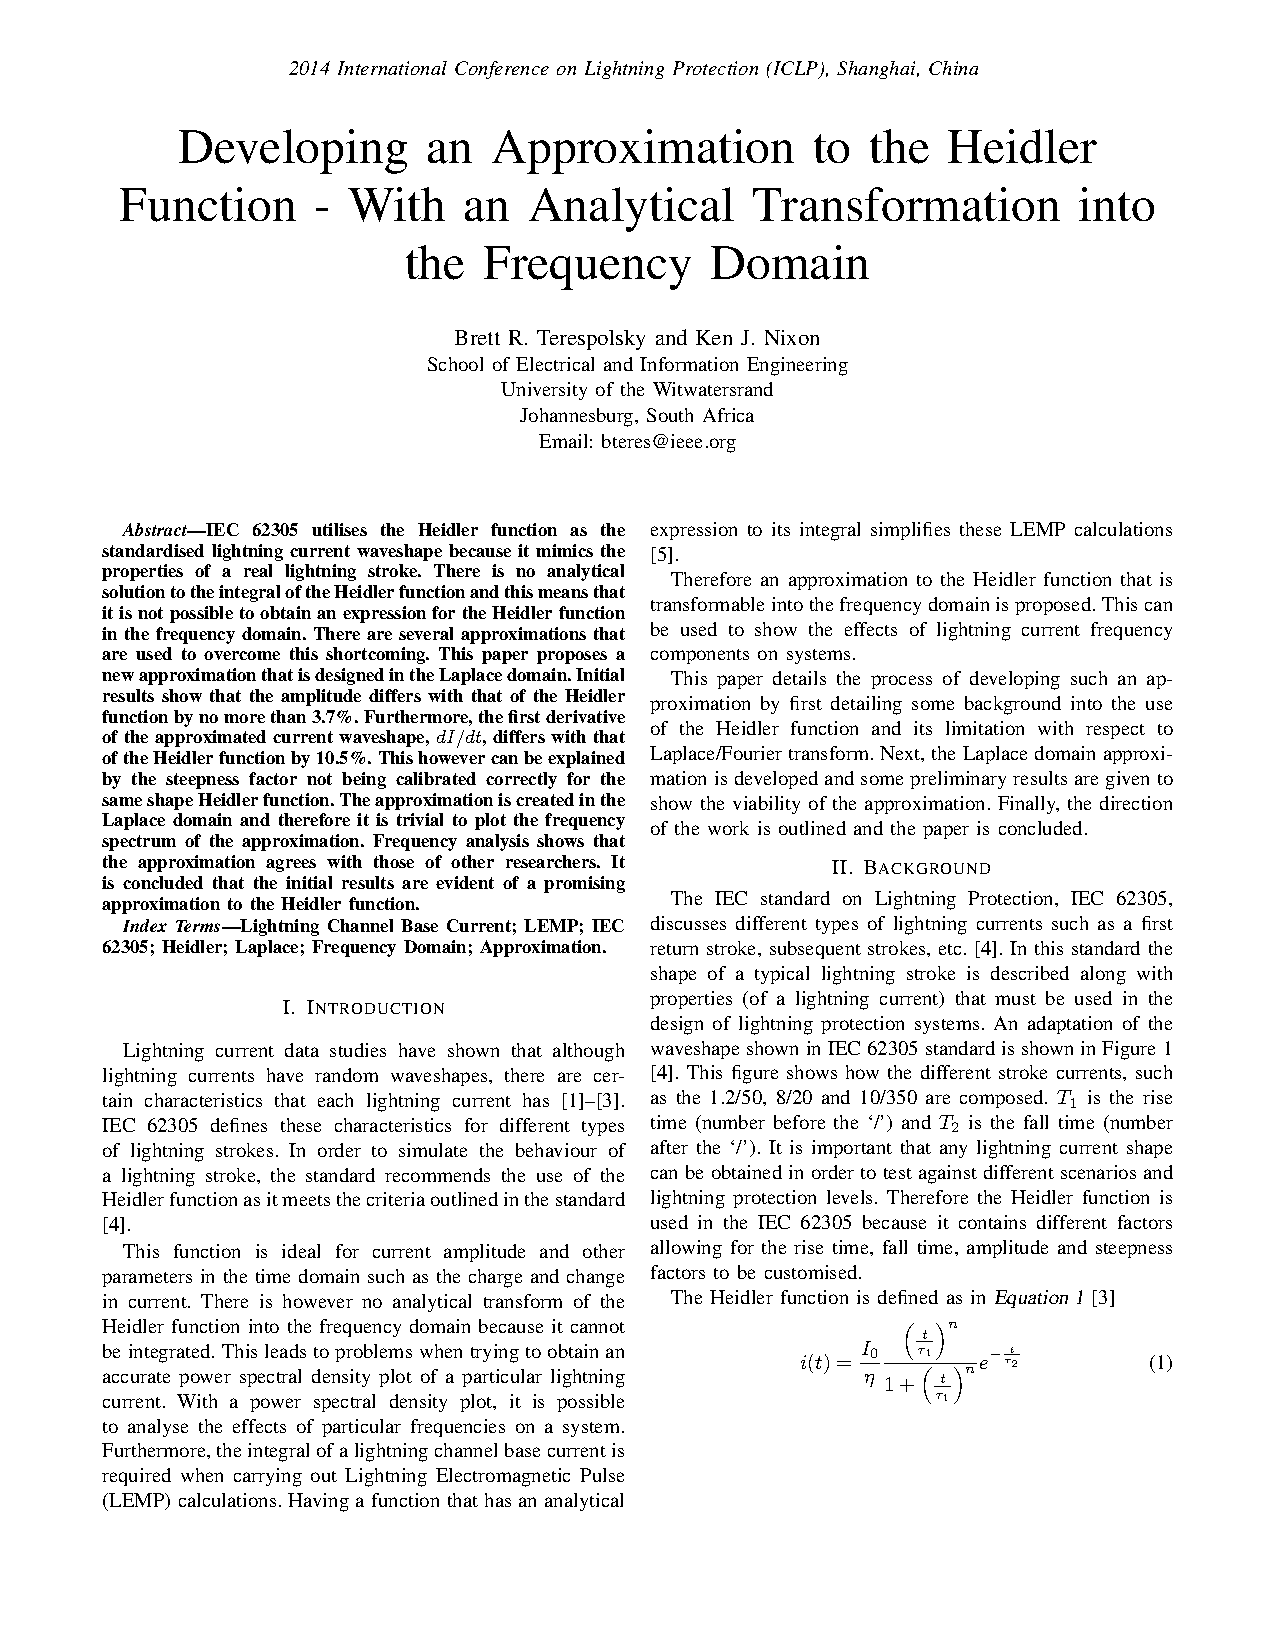
\includepdf[
  pages=-,
  width=\Gm@layoutwidth,
  height=\Gm@layoutheight,
  keepaspectratio=true
]{./AdditionalFiles/BrettTerespolskyICLP2014}
\makeatother


\addtocontents{toc}{\vspace{2em}} % Add a gap in the Contents, for aesthetics

\backmatter

%----------------------------------------------------------------------------------------
%	BIBLIOGRAPHY
%----------------------------------------------------------------------------------------

\label{Bibliography}

\lhead{\emph{References}} % Change the page header to say "Bibliography"

\bibliographystyle{IEEEtranN} % Use the "unsrtnat" BibTeX style for formatting the Bibliography
% \nocite{*}
\bibliography{Bibliographies/Bibliography} % The references (bibliography) information are stored in the file named "Bibliography.bib"

\lhead{\emph{Bibliography}}

\bibliographystylebib{apa}

\makeatletter
\def\@biblabel#1{\hspace*{-\labelsep}}
\makeatother

\bibliographybib{Bibliographies/Bibliography}
\nocitebib{*}

\end{document}
